\documentclass[a4paper 12pt]{article}

\usepackage[utf8]{inputenc}
\usepackage[T1]{fontenc}
\usepackage{mathptmx}
\usepackage{textcomp}
\usepackage[UKenglish]{babel}
\usepackage{amsmath, amssymb}
\usepackage{float}
\usepackage{xcolor}
\definecolor{codegreen}{rgb}{0,0.6,0}
\definecolor{codepurple}{rgb}{0.58,0,0.82}
\usepackage{listings}
\lstdefinestyle{code}{
	commentstyle=\color{codegreen},
	keywordstyle=\color{magenta},
	stringstyle=\color{codepurple},
	showspaces=false,
	showstringspaces=false,
	breaklines=true
}
\lstset{style=code}
\usepackage[hidelinks]{hyperref}
\hypersetup{
	colorlinks=false
}
\usepackage[style=ieee]{biblatex}
\bibliography{sources/biblio}
\renewcommand{\baselinestretch}{1.5}

\setlength{\parindent}{0pt}
\setlength{\parskip}{1em}

% figure support
\usepackage{import}
\usepackage{xifthen}
\pdfminorversion=7
\usepackage{pdfpages}
\usepackage{transparent}
\newcommand{\incfig}[1]{%
	\def\svgwidth{\columnwidth}
	\import{./figures/}{#1.pdf_tex}
}

\pdfsuppresswarningpagegroup=1

\begin{document}
\hypersetup{pageanchor=false}
\begin{titlepage}
  \begin{center}

    \textsc{\LARGE Dublin City University}\\[1cm]
    \textsc{\Large Electronic and Computer Engineering}\\[0.5cm]

    {\LARGE \bfseries EE513 Connected Embedded Systems\\[0.4cm]}
    {\Large \bfseries Assignment 1\\[0.4cm]}

    \begin{figure}[H]
	
\includegraphics{images/Dcu-logo.png}
	\centering
    \end{figure}

    \vskip 2cm
    \emph{Author}\\[0.1cm]
    \noindent\makebox[\textwidth]{%
      \begin{tabular}{ll}%
        Michael Lenehan & michael.lenehan4@mail.dcu.ie \\
	Student Number: & 15410402 \\
    \end{tabular}}\\[0.1cm]

    \vfill

    % Bottom of the page
    % Probably replaced with date of deadline
    {\large{09/03/2020}}

  \end{center}
\end{titlepage}

\hypersetup{pageanchor=true}
\pagenumbering{alph}
\thispagestyle{plain}
\begingroup
\renewcommand{\cleardoublepage}{}
\renewcommand{\clearpage}{}

\LARGE{Declaration}

\endgroup

\vskip 1cm

I declare that this material, which I now submit for assessment, is entirely my
own work and has not been taken from the work of others, save and to the extent
that such work has been cited and acknowledged within the text of my work. I
understand that plagiarism, collusion, and copying are grave and serious
offences in the university and accept the penalties that would be imposed should
I engage in plagiarism, collusion or copying. I have read and understood the
Assignment Regulations set out in the module documentation. I have identified
and included the source of all facts, ideas, opinions, and viewpoints of others
in the assignment references. Direct quotations from books, journal articles,
internet sources, module text, or any other source whatsoever are acknowledged
and the source cited are identified in the assignment references. This
assignment, or any part of it, has not been previously submitted by me or any
other person for assessment on this or any other course of study.

I have read and understood the DCU Academic Integrity and Plagiarism at
\url{https://www4.dcu.ie/sites/default/files/policy/1%20-%20integrity_and_plagiarism\_ovpaa_v3.pdf}
and IEEE referencing guidelines found at
\url{https://loop.dcu.ie/mod/url/view.php?id=448779}.

\vskip 1cm
Signed: \underline{\ \ \ \ \ \ \ \ \ \ \ \ \ \ \ \ \ \ \ \ \ \ \ \ \ \ \ \ \ \ \
\ \ \ \ \ \ } \hspace{20mm}Date: \underline{09/03/2020}

\hspace*{0mm}\phantom{Signed:}Michael Lenehan

\pagebreak

\pagenumbering{arabic}
\thispagestyle{plain}
\begin{center}
    \Large
    \textbf{Title}

    \vspace{0.4cm}
    \large
    Subtitle

    \vspace{0.4cm}
    \textbf{Michael Lenehan}

    \vspace{0.9cm}
    \textbf{Abstract}

\end{center}

\par

\pagebreak

\tableofcontents
\clearpage
\section{Introduction}
This assignment aims to introduce students to integrating physical sensors or
devices with an embedded Linux platform. In this case the physical device being
used is the DS3231 Real Time Clock module, and the embedded Linux platform is a
Raspberry Pi 3 Model B+. The devices can communicate via the I2C protocol.

The requirements of the assignment state that a C++ class must be implemented
for this integration. This class must contain all methods required for the reading
and writing of the RTC time, date, alarm, control, and temperature registers.
The student must also implement a ``novel function'' of their choosing.

In completing this assignment, the student should have a greater understanding
of the object oriented code required for I2C communications, and the code
required to read or write data to/from a physical devices registers.

\section{Conclusion}
Each of the required read and write functions of the assignment were implemented.
The novel functionality was also implemented. Documentation was created
using ``Doxygen'' and can be found in the submit git repository.

Figures \ref{fig:images-git1} and \ref{fig:images-git2} show the GitLab commit
history for the assignment. This does not demonstrate the full history of the
project, as a number of merged branches were later deleted, however all major
changes are reflected in the screenshots.

\begin{figure}[H]
	\centering
	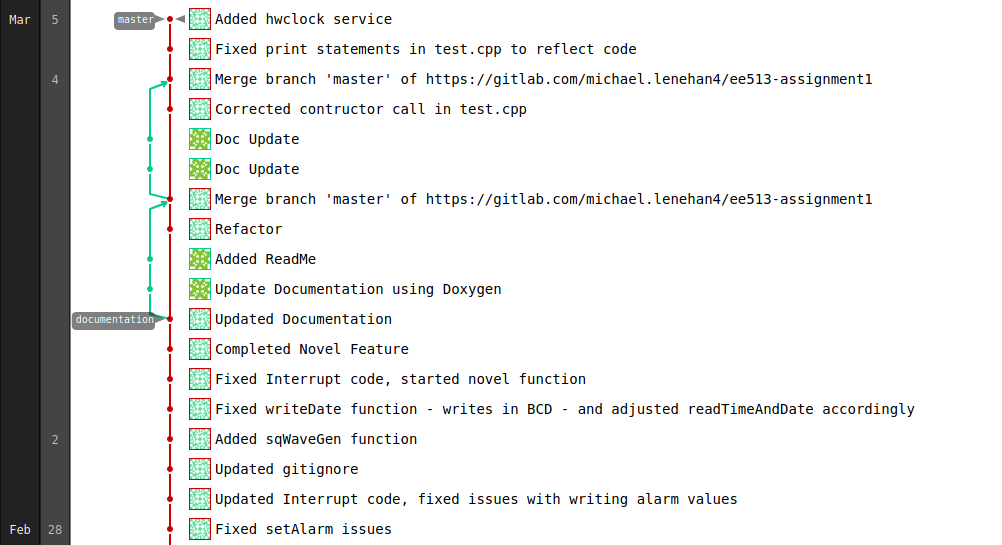
\includegraphics[width=0.8\textwidth]{images/git1}
	\caption{GitLab Commit History}
	\label{fig:images-git1}
\end{figure}

\begin{figure}[H]
	\centering
	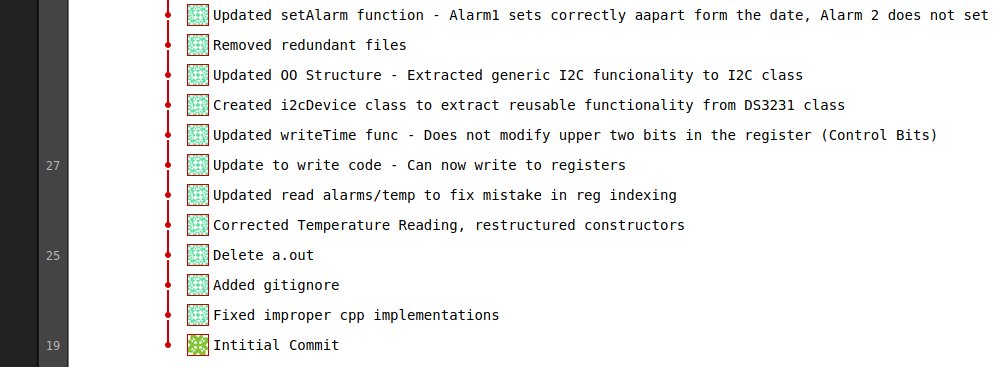
\includegraphics[width=0.8\textwidth]{images/git2}
	\caption{GitLab Commit History}
	\label{fig:images-git2}
\end{figure}

The interrupt
did not operate as expected. Reading the datasheet indicates that the interrupt
bit being set high while the alarm flag is low would result in no output on the
square wave output, however the exact opposite is true, with no output on the
pin only if the alarm flag is high.

Overall a lot was learned with regards to integrating hardware with an embedded
Linux system, including how to communicate via I2C, and how to perform
integration testing.

\clearpage
\printbibliography
\end{document}
